\documentclass[fleqn]{article}
\oddsidemargin 0.0in
\textwidth 6.0in
\thispagestyle{empty}
\usepackage{import}
\usepackage{amsmath}
\usepackage{graphicx}
\usepackage{flexisym}
\usepackage{amssymb}
\usepackage{bigints} 
\usepackage[english]{babel}
\usepackage[utf8x]{inputenc}
\usepackage{float}
\usepackage[colorinlistoftodos]{todonotes}

\definecolor{hwColor}{HTML}{AD53BA}

\begin{document}

  \begin{titlepage}

    \newcommand{\HRule}{\rule{\linewidth}{0.5mm}}

    \center


    \textsc{\LARGE Arizona State University}\\[1.5cm]

    \textsc{\LARGE Quantum Physics I }\\[1.5cm]


    \begin{figure}
      
\includegraphics[width=\linewidth]{asu.png}
    \end{figure}


    \HRule \\[0.4cm]
    { \huge \bfseries Homework Nine}\\[0.4cm] 
    \HRule \\[1.5cm]

    \textbf{Behnam Amiri}

    \bigbreak

    \textbf{Prof: Richard Kirian}

    \bigbreak


    \textbf{{\large \today}\\[2cm]}

    \vfill 

  \end{titlepage}
 
  \textbf{2.29} \\ \\
  Analyze the odd bound state wave functions for the finite square well. 
  Derive the transcendental equation for the allowed energies, and solve it
  graphically. Examine the two limiting cases. Is there always an odd bound state?

  \textcolor{hwColor}{
    \\
    Let's start with the Schr$\ddot{o}$dinger equation.
    \\
    $i\hbar \dfrac{\partial \Psi}{\partial t}=-\dfrac{\hbar^2}{2m}\dfrac{\partial^2 \Psi}{\partial x}+V(x,t) \Psi(x,t), ~~~~ -\infty<x<+\infty, ~~ t>0$ \\
    \\
    From the textbook we know that a finite square well we have:
    $$
      V(x)=\begin{cases}
        -V_0 ~~~ -a\leq x\leq +a \\
        \\
        0 ~~~~ |x|>a
      \end{cases}
    $$
    That gives us $i \hbar \dfrac{\partial \Psi}{\partial t}=-\dfrac{\hbar^2}{2m}\dfrac{\partial^2 \Psi}{\partial x}+V(x) \Psi(x,t)$ \\
    \\
    \\
    \rule{15cm}{1pt}
    \\
    \\
    \textbf{A quick review:}
    \\
    The method of separation of variables relies upon the assumption that a function of the form
    $u(x,t)=\phi(x)G(t)$ will be a solution to a linear homogeneous partial differential equation in x
    and t. This is called a product solution and provided the boundary conditions are also linear and
    homogeneous this will also satisfy the boundary conditions. The method of Separation of Variables
    cannot always be used and even when it can be used it will not always be possible to get much past
    the first step in the method.
    \\
    \rule{15cm}{1pt}
    \\
    we assume $\Psi(x,t)=\psi(x) \phi(t)$ is a solution, hence we have: \\
    \\
    $
      i\hbar \dfrac{\partial}{\partial t} \left[\psi(x) \phi(t)\right]=-\dfrac{\hbar^2}{2m}\dfrac{\partial^2}{\partial x} \left[\psi(x) \phi(t)\right]+V(x) \left[\psi(x) \phi(t)\right] \\
      \\
      \\
      i\hbar \psi(x) \phi^'(t)=-\dfrac{\hbar^2}{2m} \psi^{''}(x) \phi(t)+V(x) \psi(x) \phi(t) \\
      \\
      \\
      i\hbar \dfrac{\phi^'(t)}{\phi(t)}=-\dfrac{\hbar^2}{2m} \dfrac{\psi^{''}(x)}{\psi(x)}+V(x)
      \\
      \\
    $
      The only way a function of $t$ can be equal to a function of $x$ is if both are equal to a constant like $E$. \\
    $
      i\hbar \dfrac{\phi^'(t)}{\phi(t)}=-\dfrac{\hbar^2}{2m} \dfrac{\psi^{''}(x)}{\psi(x)}+V(x)=E \Rightarrow \begin{cases}
        E=-\dfrac{\hbar^2}{2m} \dfrac{\psi^{''}(x)}{\psi(x)}+V(x)
        \\
        \\
        E=i\hbar \dfrac{\phi^'(t)}{\phi(t)}
      \end{cases} \\
      \\
      \dfrac{d^2 \psi}{dx^2}=\dfrac{2m \psi}{\hbar}\left(V(x)-E\right) \\ \\ 
    $
    Now for the $V(x)$ intervals we have: 
    $
      \begin{cases}
        \dfrac{d^2 \psi}{dx^2}=-\dfrac{2m E \psi}{\hbar^2}, ~~~~~ |x|>a \\
        \\
        \dfrac{d^2 \psi}{dx^2}=-\dfrac{2m \psi}{\hbar^2}\left(V_0+E\right)
      \end{cases} 
    $
    \\
    \\
    \\
    The general solution is: 
    $
      \psi(x)=\begin{cases}
        C_1 ~ exp\left(\dfrac{\sqrt{-2mE}}{\hbar}x\right)+C_2 ~ exp\left(-\dfrac{\sqrt{-2mE}}{\hbar}x\right) ~~~ x<-a \\
        \\
        C_3 ~ cos\left(\dfrac{\sqrt{2m(V_0+E)}}{\hbar}x\right)+C_4 ~ sin\left(\dfrac{\sqrt{2m(V_0+E)}}{\hbar}x\right) ~~~ -a \leq x\leq +a \\
        \\
        C_5 ~ exp\left(\dfrac{\sqrt{-2mE}}{\hbar}x\right)+C_6 ~ exp\left(-\dfrac{\sqrt{-2mE}}{\hbar}x\right) ~~~ x>a 
      \end{cases}
    $
    \\
    \\
    The goal here is to find these constants. If we want $\Psi(x,t)=\psi(x) \phi(t)=0$ when $x\rightarrow \pm \infty$
    we need to set $C_2$ and $C_5$ to zero. And for the odd bound states let's set $C_3=0$ and $C_1=-C_6$. Hence we have: \\
    \\
    $
      \psi(x)=\begin{cases}
        C_1 ~ exp\left(\dfrac{\sqrt{-2mE}}{\hbar}x\right) ~~~ x<-a \\
        \\
        C_3 ~ cos\left(\dfrac{\sqrt{2m(V_0+E)}}{\hbar}x\right)+C_4 ~ sin\left(\dfrac{\sqrt{2m(V_0+E)}}{\hbar}x\right) ~~~ -a \leq x\leq +a \\
        \\
        C_6 ~ exp\left(-\dfrac{\sqrt{-2mE}}{\hbar}x\right) ~~~ x>a 
      \end{cases} \\
      \\
      \\
      \lim\limits_{x \to \pm a^-}=\lim\limits_{x \to \pm a^+} \Rightarrow C_4 ~ sin\left(\dfrac{\sqrt{2m(V_0+E)}}{\hbar}a\right)=C_6 ~ exp\left(-\dfrac{\sqrt{-2mE}}{\hbar}a\right) \\
      \\
      \Longrightarrow C_6=C_4  sin\left(\dfrac{\sqrt{2m(V_0+E)}}{\hbar}a\right) ~ exp\left(\dfrac{\sqrt{-2mE}}{\hbar}a\right)
    $
    \\
    \\
    Therefore, the odd bound state for the finite square well: \\
    \\
    $
      \psi(x)=\begin{cases}
        -C_4  sin\left(\dfrac{\sqrt{2m(V_0+E)}}{\hbar}a\right) ~ exp\left(\dfrac{\sqrt{-2mE}}{\hbar}(x+a)\right) ~~~ x<-a \\
        \\
        C_4 ~ sin\left(\dfrac{\sqrt{2m(V_0+E)}}{\hbar}x\right) ~~~ -a \leq x\leq +a \\
        \\
        C_4  sin\left(\dfrac{\sqrt{2m(V_0+E)}}{\hbar}a\right) ~ exp\left(-\dfrac{\sqrt{-2mE}}{\hbar}(x-a)\right) ~~~ x>a 
      \end{cases}
    $
    \\
    \\
    The time-independent Schr$\ddot{o}$dinger equation is homogeneous meaning $C_4$ can be anything but if we
    choice it wisely so that $\psi^2(x)=1$. \\
    \\
    \\
    $
      \bigints_{-\infty}^{+\infty} \left[\psi(x)\right]^2 dx=\bigints_{-\infty}^{-a} \left[\psi(x)\right]^2 dx+\bigints_{-a}^{+a} \left[\psi(x)\right]^2 dx+ \bigints_{+a}^{+\infty} \left[\psi(x)\right]^2 dx
      \\
      \\
      =\bigints_{-\infty}^{-a} \left[-C_6 ~ exp\left(\dfrac{\sqrt{-2mE}}{\hbar}x\right)\right]^2 dx
      +\bigints_{-a}^{+a} \left[C_4 ~ sin\left(\dfrac{\sqrt{2m(V_0+E)}}{\hbar}x\right)\right]^2 dx
      +\bigints_{+a}^{+\infty} \left[C_6 ~ exp\left(-\dfrac{\sqrt{-2mE}}{\hbar}x\right)\right]^2 dx
      \\
      \\
      \\
      =C^2_6 \bigints_{-\infty}^{-a} exp\left(2\dfrac{\sqrt{-2mE}}{\hbar}x\right) dx
      +C^2_4 \bigints_{-a}^{+a} sin^2\left(\dfrac{\sqrt{2m(V_0+E)}}{\hbar}x\right) dx
      +C^2_6 \bigints_{+a}^{+\infty} exp\left(-2\dfrac{\sqrt{-2mE}}{\hbar}x\right) dx
      \\
      \\
      \\
      =C^2_6 \left[\dfrac{\hbar}{2\sqrt{-2mE}} ~ exp\left(\dfrac{2x\sqrt{-2mE}}{\hbar}\right) \Bigg|_{-\infty}^{-a}\right] \\
      +C^2_4 \left[ x-\dfrac{\hbar}{2\sqrt{2m(V_0+E)}} sin\left( \dfrac{2x\sqrt{2m(V_0+E)}}{\hbar}\right)\Bigg|_{0}^{a}\right] \\
      +C^2_6 \left[-\dfrac{\hbar}{2\sqrt{-2mE}} ~ exp\left(-\dfrac{2x\sqrt{-2mE}}{\hbar}\right) \Bigg|_{+a}^{+\infty}\right] 
    $ \\
    \\
    \\
    By doing some algebra we have: \\
    \\
    \\
    $
      \therefore ~~~ C_4=\dfrac{1}{\sqrt{a+\dfrac{\hbar}{\sqrt{-2mE}} sin^2 \left(\dfrac{a\sqrt{2m(V_0+E)}}{\hbar}\right)-\dfrac{\hbar}{2\sqrt{2m (V_0+E)}} sin\left(\dfrac{2a\sqrt{2m(V_0+E)}}{\hbar}\right)}} ~~~~ \surd
    $ 
    \\
    \\
    The energy corresponding to the eigenstate $\psi(x)$: \\
    \\
    \\
    $
      \bigints_{a-\epsilon}^{a+\epsilon} \dfrac{d^2 \psi}{dx^2} dx=\bigints_{a-\epsilon}^{a+\epsilon} \dfrac{2m \psi(x)}{\hbar^2} \left(V(x)-E\right) dx \\
      \\
      \\
      \dfrac{d\psi}{dx} \Bigg|_{a-\epsilon}^{a+\epsilon}=\bigints_{a-\epsilon}^{a} \dfrac{2m \psi(x)}{\hbar^2} \left(-V_0-E\right) dx-\bigints_{a}^{a+\epsilon} \dfrac{2m \psi(x) E}{\hbar^2} dx=-\dfrac{2m \psi(a) \epsilon}{\hbar^2} \left(V_0+E\right)-\dfrac{2m \psi(a)E}{\hbar^2} 
    $
    \\
    \\
    Taking the limit $\epsilon \to 0$ \\
    \\
    \\
    $
      \therefore ~~~ \dfrac{d\psi}{dx} \Bigg|_{a-}^{a+}=0 ~~~ \surd \\
      \\
      \\
      \\
      \lim\limits_{x\to a^-} \dfrac{d\psi}{dx}=\lim\limits_{x\to a^+} \dfrac{d\psi}{dx}: 
      C_4\dfrac{\sqrt{2m(V_0+E)}}{\hbar} cos\left(\dfrac{\sqrt{2m(V_0+E)}a}{\hbar}\right)=-C_4 sin\left(\dfrac{\sqrt{2m(V_0+E)}}{\hbar}a\right) \left(\dfrac{\sqrt{-2mE}}{\hbar}\right)
      \\
      \\
      \\
      \Longrightarrow -\dfrac{\sqrt{2m(V_0+E)}}{\hbar} ~ cot\left(\dfrac{\sqrt{2m(V_0+E)}}{\hbar}a\right)=\dfrac{\sqrt{-2mE}}{\hbar}
      \\
      \\
      \\
      -a\dfrac{\sqrt{2m(V_0+E)}}{\hbar} ~ cot\left(\dfrac{\sqrt{2m(V_0+E)}}{\hbar}a\right)=a\dfrac{\sqrt{-2mE}}{\hbar} \\
      \\
      \\
      -a\dfrac{\sqrt{2m(V_0+E)}}{\hbar} ~ cot\left(\dfrac{\sqrt{2m(V_0+E)}}{\hbar}a\right)=a\left[\sqrt{\dfrac{2mV_0}{\hbar^2}-\dfrac{2m(V_0+E)}{\hbar^2}}\right] \\
      \\
      \\
      -a\dfrac{\sqrt{2m(V_0+E)}}{\hbar} ~ cot\left(\dfrac{\sqrt{2m(V_0+E)}}{\hbar}a\right)=\sqrt{\left(\dfrac{a\sqrt{2mV_0}}{\hbar}\right)^2-\left(\dfrac{a\sqrt{2m(V_0+E)}}{\hbar}\right)^2} \\
      \\
      \\
      \begin{cases}
        z_0 \equiv \dfrac{a\sqrt{2mV_0}}{\hbar} \\
        \\
        z \equiv \dfrac{a\sqrt{2m(V_0+E)}}{\hbar}
      \end{cases} \Longrightarrow -z cot(z)=\sqrt{z^2_0-z^2} 
      \\
      \\
      \\
      \therefore ~~~ -cot(z)=\sqrt{\left(\dfrac{z_0}{z}\right)^2-1} ~~~ \surd 
    $
    \\
    \\
    \\
    \\
    \\
    \\
    \\
    \\
    \\
    \emph{The number of intersections indicates the number of legitimate odd bound states.}
    \\
    When $z_0$ is at $\dfrac{\pi}{2}$ then there is one intersection at $z=\dfrac{\pi}{2}$
    \\
    \\
    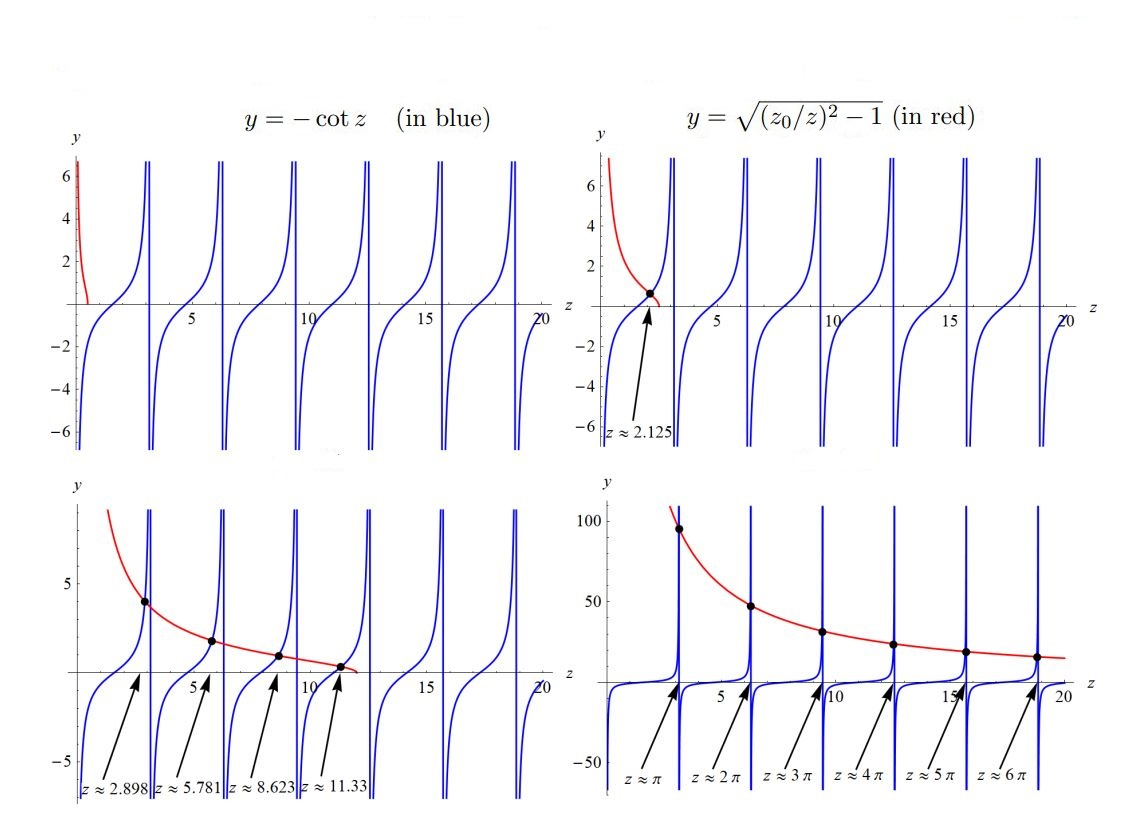
\includegraphics[height=8cm, width=16cm]{two.JPG} \\
    \\
    \\
    $
      z_0=\dfrac{a\sqrt{2mV_0}}{\hbar} < \dfrac{\pi}{2} \Longrightarrow V_0 < \dfrac{\pi^2 \hbar^2}{8ma^2} \\
      \\
    $
    While $V_0$ is less than that there are no odd bound states. \\
    $  
      \\
      z=\dfrac{a\sqrt{2m(V_0+E)}}{\hbar} \approx n\pi \Longrightarrow V_0+E_n \approx \dfrac{\pi^2 \hbar^2(2n)^2}{8ma^2}
    $
    \\
    \\
    Since $\dfrac{\partial \Psi}{\partial x}$ at $x=a$, then we have: \\
    \\
    \\
    $
      \lim\limits_{x\to a^-} \dfrac{d\psi}{dx}=\lim\limits_{x\to a^+} \dfrac{d\psi}{dx}: 
      C_4\dfrac{\sqrt{2m(V_0+E)}}{\hbar} cos\left(\dfrac{\sqrt{2m(V_0+E)}a}{\hbar}\right)=-C_4 sin\left(\dfrac{\sqrt{2m(V_0+E)}}{\hbar}a\right) \left(\dfrac{\sqrt{-2mE}}{\hbar}\right) \\
      \\
      \\
      \dfrac{\hbar}{\sqrt{-2mE}} cos \left(a\dfrac{\sqrt{2m(V_0+E)}}{\hbar}\right)=-\dfrac{\hbar}{\sqrt{2m(V_0+E)}} sin\left(\dfrac{a\sqrt{2m(V_0+E)}}{\hbar}\right) \\
      \\
      \\
      \\
      C_4=\dfrac{1}{\sqrt{a+\dfrac{\hbar}{\sqrt{-2mE}} sin^2 \left(\dfrac{a\sqrt{2m(V_0+E)}}{\hbar}\right)-\dfrac{\hbar}{2\sqrt{2m (V_0+E)}} sin\left(\dfrac{2a\sqrt{2m(V_0+E)}}{\hbar}\right)}} \\
      \\
      \\
      =\dfrac{1}{\sqrt{a+\dfrac{\hbar}{\sqrt{-2mE}} sin^2 \left(\dfrac{a\sqrt{2m(V_0+E)}}{\hbar}\right)-\dfrac{\hbar}{2\sqrt{2m (V_0+E)}} sin\left(\dfrac{a\sqrt{2m(V_0+E)}}{\hbar} \right) cos\left(\dfrac{a\sqrt{2m(V_0+E)}}{\hbar}\right)}} \\
      \\
      \\
      =\dfrac{1}{\sqrt{a+\dfrac{\hbar}{\sqrt{-2mE}} sin^2 \left(\dfrac{a\sqrt{2m(V_0+E)}}{\hbar}\right)+\dfrac{\hbar}{\sqrt{-2mE}} cos^2\left(\dfrac{a\sqrt{2m(V_0+E)}}{\hbar}\right)}} \\
      \\
      \\
      \\
      \therefore ~~~ C_4=\dfrac{1}{\sqrt{a+\dfrac{\hbar}{\sqrt{-2mE}}}} ~~~ \surd \\
      \\
      \\
      \\
    $
    The odd bound state is: \\
    \\
    \\
    $
      \psi(x)=\begin{cases}
        -\dfrac{1}{\sqrt{a+\dfrac{\hbar}{\sqrt{-2mE}}}}  sin\left(\dfrac{\sqrt{2m(V_0+E)}}{\hbar}a\right) ~ exp\left(\dfrac{\sqrt{-2mE}}{\hbar}(x+a)\right) ~~~ x<-a \\
        \\
        \dfrac{1}{\sqrt{a+\dfrac{\hbar}{\sqrt{-2mE}}}} ~ sin\left(\dfrac{\sqrt{2m(V_0+E)}}{\hbar}x\right) ~~~ -a \leq x\leq +a \\
        \\
        \dfrac{1}{\sqrt{a+\dfrac{\hbar}{\sqrt{-2mE}}}}  sin\left(\dfrac{\sqrt{2m(V_0+E)}}{\hbar}a\right) ~ exp\left(-\dfrac{\sqrt{-2mE}}{\hbar}(x-a)\right) ~~~ x>a 
      \end{cases}
    $
  }

  \pagebreak

  \textbf{2.31} \\ \\
  The Dirac delta function can be thought of as the limiting case of a
  rectangle of area 1, as the height goes to infinity and the width goes to zero. Show
  that the delta-function well (Equation 2.117) is a "weak" potential (even though it
  is infinitely deep), in the sense that $z \rightarrow 0$. Determine the bound state energy
  for the delta-function potential, by treating it as the limit of a finite square well.
  Check that your answer is consistent with Equation 2.132. Also show that
  Equation 2.172 reduces to Equation 2.144 in the appropriate limit.

    \textcolor{hwColor}{
      From the textbook we have. \\
      \\
      $
        \begin{cases}
          V(x)=-\alpha \delta(x) ~~~~~~~~~~~~~~ (2.117) \\
          \\
          \psi(x)=\dfrac{\sqrt{m \alpha}}{\hbar} e^{-m \alpha |x|/\hbar^2}; E=-\dfrac{m \alpha^2}{2\hbar^2} ~~~~~~~~~~~~~~ (2.132) \\
          \\
          T^{-1}=1+\dfrac{V^2_0}{4E(E+V_0)} ~ sin^2 \left(\dfrac{2a}{\hbar} \sqrt{2m(E+V_0)}\right) ~~~~~~~~~~~~~~ (2.172)
        \end{cases}
      $
      \\
      \\
      We got the square well potential as 
      $
        \begin{cases}
          0 ~~~~~ x<-a \\
          \\
          -V_0 ~~~~~ -a\leqslant x \leqslant +a \\
          \\
          0 ~~~~~ x>a
        \end{cases}
      $ \\
      \\
      \\
      We are asked to show the delta-function well is a weak potential as $z \to 0$. Let's start with
      equation (2.117). 
      \\ 
      \\
      $
        V(x)=-\alpha \delta(x), ~~~~ V_0 \equiv \dfrac{\alpha}{\epsilon}, ~~~~ \alpha=\dfrac{\epsilon}{2}
      $ \\
      \\
      \\
      We have $z_0=\dfrac{a \sqrt{2mV_0}}{\hbar}=\dfrac{1}{\hbar}\sqrt{\dfrac{m \alpha \epsilon}{2}}$ \\ \\
      Taking the limit as $\epsilon \to 0$ we get $\lim\limits_{\epsilon \to 0} z_0=0$. \\
      \\
      \\
      We just showed \emph{the delta-function well is a weak potential}. \\
      \\
      \\
      \textbf{The bound state energy for the delta-function potentia}: \\
      \\
      \\
      $
        tan(z)=\sqrt{(\dfrac{z_0}{z})^2-1} \\ \\
        \begin{cases}
          z_0=\dfrac{a \sqrt{2mV_0}}{\hbar} \\
          \\
          z=\dfrac{a\sqrt{2m(E+V_0)}}{\hbar}
        \end{cases}
        \Longrightarrow tan(\dfrac{a\sqrt{2m(E+V_0)}}{\hbar})=\sqrt{(\dfrac{\dfrac{a \sqrt{2mV_0}}{\hbar}}{\dfrac{a\sqrt{2m(E+V_0)}}{\hbar}})^2-1}
        =\sqrt{\dfrac{V_0}{V_0+E}+1}
      $
      \\
      \\
      Based on the variables $\alpha$ and $\epsilon$ that we defined earlier, we can rewrite the above result as: 
      \\
      \\
      $
        tan\left(\dfrac{\epsilon \sqrt{2m(E+\alpha/\epsilon)}}{2\hbar}\right)=\sqrt{\dfrac{\dfrac{\alpha}{\epsilon}}{E+\dfrac{\alpha}{\epsilon}}-1}
      $
      \\
      \\
      We know from calculus that when $\theta$ is very small then $tan(\theta) \approx \theta$, with that said,
      we have: \\
      \\
      \\
      $
        \dfrac{1}{\hbar}=\sqrt{\dfrac{\alpha m \epsilon}{2}}=\sqrt{\dfrac{1}{\dfrac{\epsilon E}{\alpha}+1}-1} \Longrightarrow 
        E=-\dfrac{m \alpha^2}{\epsilon m \alpha+2\hbar^2} \\
        \\
        \\
        \lim\limits_{\epsilon \to 0} E=\lim\limits_{\epsilon \to 0} \left(-\dfrac{m \alpha^2}{\epsilon m \alpha+2\hbar^2} \right) \\
        \\
        \\
        \\
        \therefore ~~~~ E=-\dfrac{m}{2} \left(\dfrac{\alpha}{\hbar}\right)^2 ~~~ \surd
      $
      \\
      \\
      What we just found is the energy of the bound state for $V(x)=-\alpha \delta(x)$ which is the same 
      equation as 2.132 from the textbook.  \\
      \\
      \\
      \\
      Now it is time to show that equation 2.172 reduces to equation 2.144. \\
      \\
      \\
      $
        T^{-1}=1+\dfrac{V^2_0}{4E(E+V_0)} ~ sin^2 \left(\dfrac{2a}{\hbar} \sqrt{2m(E+V_0)}\right) \\
        \\
        \\
        T^{-1}=1+\dfrac{\left(\dfrac{\alpha}{\epsilon}\right)^2}{4E(E+\dfrac{\alpha}{\epsilon})} sin^2\left(\dfrac{\epsilon}{\hbar} \sqrt{2m\left(E+\dfrac{\alpha}{\epsilon}\right)} \right)
        =1+\dfrac{  \alpha^2 sin^2 \left(  \dfrac{1}{\hbar}  \sqrt{2mE \epsilon^2+2m\alpha \epsilon}  \right)  }{4 \epsilon^2 E^2 +4 \epsilon \alpha E}
        \approx 1+\dfrac{\alpha^2 sin^2\left(\dfrac{1}{\hbar} \sqrt{2m\epsilon \alpha}\right)}{4E \epsilon \alpha}
      $ \\
      \\
      \\
      Since $sin(\theta) \approx \theta$ for very small angles, hence: \\
      \\
      $
        T^{-1}=1+\dfrac{\alpha^2 sin^2\left(\dfrac{1}{\hbar} \sqrt{2m\epsilon \alpha}\right)}{4E \epsilon \alpha}
        =1+\dfrac{\alpha^2}{4E\epsilon \alpha} \left(\dfrac{1}{\hbar} \sqrt{2m\alpha \epsilon}\right)^2
        =1+\dfrac{\alpha}{4 \epsilon E} \left(\dfrac{2m \epsilon \alpha}{\hbar^2}\right) 
        =1+\dfrac{\alpha^2 m}{2\hbar^2 E} \\
        \\
        \\
        \therefore ~~~~ T=\dfrac{1}{1+\left(\dfrac{m \alpha^2}{2\hbar^2 E}\right)} ~~~~ \surd
      $  \\
      \\
      \\
      We just showed that equation 2.172 reduces to equation 2.144.
    }

  \rule{15cm}{1pt}
  
  \textbf{2.33} \\ \\
  Determine the transmission coefficient for a rectangular barrier
  (same as Equation 2.148, only with $V(x)=+V_0 >0$ in the region $-a<x<a$).
  Treat separately the three cases $E<V_0, ~ E=V_0, ~ $ and $E>V_0$ 
  (note that the wave function inside the barrier is different in the three cases).
  Partial answer: for $E<V_0$
  $$T^{-1}=1+\dfrac{V^2_0}{4E(V_0-E)} sinh^2 \left(\dfrac{2a}{\hbar} \sqrt{2m(V_0-E)}\right)$$


  \rule{15cm}{1pt}
  
  \textbf{2.40} \\ \\
  A particle of mass m in the harmonic oscillator potential (Equation
  2.44) starts out in the state
  $$\Psi(x,0)=A \left(1-2\sqrt{\dfrac{m \omega}{\hbar}}x\right)^2 ~ e^{-\dfrac{m\omega}{2\hbar} x^2}$$
  for some constant $A$.
  \begin{itemize}
    \item Determine $A$ and the coefficients $c_n$ in the expansion of this state in terms
    of the stationary states of the harmonic oscillator.

    \item In a measurement of the particle’s energy, what results could you get, and
    what are their probabilities? What is the expectation value of the energy?

    \item At a later time T the wave function is
    $$\Psi(x,T)=B\left(1+2\sqrt{\dfrac{m \omega}{\hbar}}x\right)^2 ~ e^{-\dfrac{m\omega}{2\hbar} x^2}$$
    for some constant B. What is the smallest possible value of $T$?
  \end{itemize}


  \rule{15cm}{1pt}
  
  \textbf{2.58} \\ \\
  In a monovalent metal, one electron per atom is free to roam
  throughout the object. What holds such a material together—why doesn’t it
  simply fall apart into a pile of individual atoms? Evidently the energy of the
  composite structure must be less than the energy of the isolated atoms. This
  problem offers a crude but illuminating explanation for the cohesiveness of
  metals.
  \begin{itemize}
    \item Estimate the energy of N isolated atoms, by treating each one as an
    electron in the ground state of an infinite square well of width a
    (Figure 2.23(a)).
    
    \item When these atoms come together to form a metal, we get N electrons in a
    much larger infinite square well of width Na (Figure 2.23(b)). Because of
    the Pauli exclusion principle (which we will discuss in Chapter 5) there
    can only be one electron (two, if you include spin, but let’s ignore that) in
    each allowed state. What is the lowest energy for this system
    (Figure 2.23(b))?

    \item The difference of these two energies is the \textbf{cohesive energy} of the metal—
    the energy it would take to tear it apart into isolated atoms. Find the
    cohesive energy per atom, in the limit of large N.


    \item Atypical atomic separation in a metal is a few Ångström (say, $a \approx 4 ~ \mbox{\normalfont\AA}$).
    What is the numerical value of the cohesive energy per atom, in this
    model? (Measured values are in the range of 2–4 eV.)

    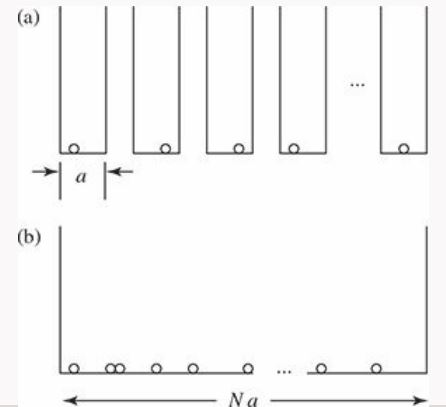
\includegraphics[height=6cm, width=10cm]{one.JPG}
    
  \end{itemize}


  \end{document}
